\chapter{Bath Observables in NMQSD and HOPS}%
\label{chap:flow}
After setting the stage for open systems and introducing the prime
tools of this work, the NMQSD and HOPS, in \cref{chap:intro}, we will
now return to our original goal, the calculation of bath related
quantities. Although the NMQSD is a method for the reduced system
state, we still treat the full unitary dynamics of system and bath and
may expect that some information about the bath is retained.

In \cref{sec:flow_lin} we will begin by deriving an expression for the
bath energy change \(-∂_{t}\ev{H_{B}}\). Subsequently we will
generalize this result to the nonlinear theory in
\cref{sec:nonlin_flow} and to finite temperatures in
\cref{sec:lin_finite}. Yet a more general class of observables can be
treated with the methods that will be developed as is shown in
\cref{sec:general_obs}.

The generalization to multiple baths in \cref{sec:multibath} and time
dependent Hamiltonians in \cref{sec:timedep} will present itself as
straight forward.

\section{Bath Energy Change of a Zero Temperature Bath}%
\label{sec:flow_lin}

In this section we demonstrate upon the example of the change of the
bath energy
\begin{equation}
  \label{eq:heatflowdef}
  J = - \dv{\ev{H_\bath}}{t}
\end{equation}
how collective bath observables may be obtained from the formalism
presented in \cref{sec:nmqsd_basics,sec:hops_basics}. We have adorned
\cref{eq:heatflowdef} with a negative sign and henceforth call this
quantity the bath energy flow or simply flow, as it constitutes the
flow of energy out of the bath into system and interaction.

The simplest version of the general model \cref{eq:generalmodel} is
given by
\begin{equation}
  \label{eq:totalH}
  H = H_\sys + \underbrace{LB^† + L^† B}_{H_\inter} + H_\bath
\end{equation}
with the system hamiltonian \(H_\sys\), the bath Hamiltonian
\(H_\bath = ∑_\lambda ω_\lambda a_{λ}^† a_{λ}\), the bath coupling
system operator \(L\) and the bath coupling bath operator
\(B=∑_{\lambda} g_{\lambda} a_{\lambda}\) which define the interaction
Hamiltonian \(H_\inter\).

We do not consider external modulation of the Hamiltonian, finite
temperatures or multiple baths at this stage, as we are interested in
the essentials of the procedure. With this approach we also follow the
``historical'' order of derivation.

Working, for now, in the Schr\"odinger picture, the Ehrenfest theorem
can be employed to find
\begin{equation}
  \label{eq:ehrenfest}
  \i∂_t\ev{H_\bath} = \ev{[H_\bath,H]} = \ev{[H_\bath,H_\inter]}.
\end{equation}
Thus, we need to calculate
\begin{eqnarray}
  \label{eq:calccomm}
    [H_\bath,H_\inter] = L[H_\bath, B^† ] - \hc.
\end{eqnarray}
This checks out as the commutator has to be anti-hermitian due to
\cref{eq:ehrenfest}.
Using \([H_\bath, B^† ]=∑_\lambda ω_\lambda g^\ast_\lambda
a^†_\lambda\) it follows that
\begin{equation}
  \label{eq:expcomm}
  \begin{aligned}
    \ev{[H_\bath,H_\inter]} &= ∑_\lambda ω_\lambda g^\ast_\lambda
    \ev{La^†_\lambda} - \cc
    = ∑_\lambda ω_\lambda g^\ast_\lambda
    \ev{La^†_\lambda \eu^{\i ω t}}_\inter - \cc\\
    &= \frac{1}{\i}\ev{L∂_t{∑_\lambda
        g^\ast_\lambda a^†_\lambda \eu^{\i ω t}}}_\inter - \cc
    =\frac{1}{\i}\qty(\ev{L\dot{B}^†}_\inter  + \cc)
  \end{aligned}
\end{equation}
where we switched to the interaction picture with respect to \(H_\bath\)
in keeping with the standard NMQSD formalism.
In essence this is just the Heisenberg equation for \(H_\inter\). The
expression for \(J\) follows
\begin{equation}
  \label{eq:final_flow}
  J(t) = \ev{L^† \dot{B}(t) + L\dot{B}^†(t)}_\inter.
\end{equation}

From this point on, we will assume the interaction picture and drop
the \(I\) subscript. The two summands yield different expressions when
evaluated in terms of the NMQSD.

For use with HOPS with the final goal of utilizing the auxiliary
states, the expression \(\ev{L^†∂_t B(t)}\) should be evaluated.  We
calculate
\begin{equation}
  \label{eq:interactev}
  \ev{L^†∂_t B(t)}=\ev{L^†∂_t B(t)}{\psi(t)} =
  ∫ \braket{\psi(t)}{\vb{z}}\mel{\vb{z}}{L^†∂_tB(t)}{\psi(t)}\frac{\dd[2]{\vb{z}}}{\pi^N},
\end{equation}
where \(N\) is the total number of environment oscillators and
\(\vb{z}=\qty(z_{\lambda_1}, z_{\lambda_2}, \ldots)\).

Using
\(\mel{\vb{z}}{a_λ}{ψ}= ∂_{z^\ast_λ}\braket{\vb{z}}{ψ}=
∂_{z^\ast_λ}\ket{ψ(\vb{z}^\ast,t)}\) and
\(\mel{\vb{z}}{a_λ^\dag}{ψ}= z_λ^\ast\ket{ψ(\vb{z}^\ast,t)}\) we find
\begin{equation}
  \label{eq:nmqsdficate}
  \begin{aligned}
    \mel{z}{∂_tB(t)}{\psi(t)} &= ∑_\lambda g_\lambda
  \qty(∂_t \eu^{-\iω_\lambda
    t})∂_{z^\ast_\lambda}\ket{\psi(z^\ast,t)} \\
  &= ∫_0^t ∑_\lambda g_\lambda
  \qty(∂_t \eu^{-\iω_\lambda
    t})\pdv{η_s^\ast}{z^\ast_\lambda}\fdv{\ket{\psi(z^\ast,t)}}{η^\ast_s}\dd{s}\\
  &= -\i∫_0^t\dot{\alpha}(t-s)\fdv{\ket{\psi(η^\ast_{t},t)}}{η^\ast_s}\dd{s},
  \end{aligned}
\end{equation}
where
\(η^\ast_t\equiv -\i ∑_\lambda g^\ast_\lambda z^\ast_\lambda
\eu^{\iω_\lambda t}\) which led to the chain rule
\(∂_{z^\ast_λ}=∫\dd{s}\pdv{η_s^\ast}{z^\ast_λ}\fdv{}{η_s^\ast}\)
exactly corresponding to the procedure in
\cref{sec:nmqsd_basics}.

With this we obtain
\begin{equation}
  \label{eq:steptoproc}
  \ev{L^†∂_t B(t)} = -\i \mathcal{M}_{η^\ast}\bra{\psi(η_{t},
    t)}L^†∫_0^t\dd{s} \dot{\alpha}(t-s)\fdv{η^\ast_s} \ket{\psi(η^\ast_{t},t)}.
\end{equation}
Defining
\begin{equation}
  \label{eq:defdop}
D_t = ∫_0^t\dd{s} \alpha(t-s)\fdv{η^\ast_s}
\end{equation}
as in \refcite{Suess2014Oct} we find
\begin{equation}
  \label{eq:final_flow_nmqsd}
  J(t) = -\i \mathcal{M}_{η^\ast}\bra{\psi(η,
    t)}L^†\dot{D}_t\ket{\psi(η^\ast,t)} + \cc,
\end{equation}
where we have used that the integral in \(D_t\) can be expanded over the
whole real axis. If we assume \(\alpha = \exp(-w t)\) then
\begin{equation}
  \label{eq:hopsj}
  J(t) = \i \mathcal{M}_{η^\ast}\bra{\psi^{(0)}(η,
    t)}wL^†\ket{\psi^{(1)}(η^\ast,t)} + \cc.,
\end{equation}
where \(\ket{\psi^{(1)}(η^\ast,t)}\) is the first HOPS hierarchy
state. This can be generalized to any BCF that is a sum of exponentials.

Interestingly one finds that
\begin{equation}
  \label{eq:alternative}
  \ev{L∂_t B^†(t)} = \i \mathcal{M}_{η^\ast}
  \dot{η}_t^\ast \mel{\psi(η,t)}{L}{\psi(η^\ast,t)}.
\end{equation}
This expression is undesirable as it does not exist for all bath
correlation functions\footnote{Only for BCFs that are smooth at
  \(τ=0\).} and expressions involving the process directly are alleged
to converge more slowly, especially for shorter bath memories. This
convergence problem is due to greater magnitude and shorter
correlation time of the oscillations of \(\dot{η}_{t}^\ast\), as can
be seen in \cref{fig:stocproc_comparison}.
\begin{figure}[htp]
  \centering
  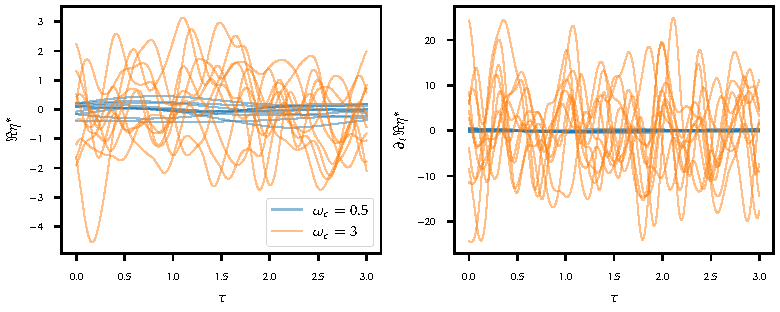
\includegraphics{figs/analytic_comp/stocproc_comparison}
  \caption{\label{fig:stocproc_comparison} The imaginary part of ten
    realizations of the stochastic process \(η^\ast\) for an ohmic BCF
    with different cutoff frequencies \(ω_{c}\). The process is much
    smoother and of less magnitude for smaller cutoffs. The difference
    between the cutoffs is even more severe for the derivative of the
    processes.}
\end{figure}
The derivative of the process is correlated according to
\(\ev{η_{t}η^\ast_{s}}=\ddot{α}(t-s)\) which has a greater magnitude
at \(τ=0\) and falls off faster in the Ohmic case.

Furthermore, this approach becomes more complicated in the nonlinear
theory due to the shift of the stochastic process.  We will briefly
return to this issue in \cref{sec:general_obs}.

In the language of \cref{sec:hops_basics} we can generalize to
\(\alpha(t) = ∑_i G_i \eu^{-W_i t}\) obtaining
\begin{equation}
  \label{eq:hopsflowfock}
  J(t) = - ∑_\mu\sqrt{G_\mu}W_\mu
  \mathcal{M}_{η^\ast}\bra{\psi^{(0)}(η,
    t)}L^†\ket{\psi^{\vb{e}_\mu}(η^\ast,t)} + \cc,
\end{equation}
where \(\ket{\psi^{\vb{e}_\mu}(η^\ast,t)}\) are the first hierarchy
states.

Note however, that it is not primarily the first hierarchy states that
contain the information about the bath. Looking at
\cref{eq:alternative}, we would require only the zeroth hierarchy
states and the stochastic process. The latter is no product of the
actual dynamics, but due to the choice of a concrete \(\vb{z}\) in
\cref{eq:interactev}. The bath information is discarded, when
averaging over all stochastic processes, as this is equivalent to
tracing out the bath. The crucial point here is, that we have hooked
into the formalism before the trace is performed, still having access
to the global state. The averaging in \cref{eq:final_flow_nmqsd} then
discards all the information about the bath that we don't need.

Now that we have covered the simplest case, we will endeavor to make
the result useful in practice.

\section{Generalization to the Nonlinear Theory}
\label{sec:nonlin_flow}
Due to the inferior convergence of the linear method for stronger
coupling \cite{Suess2014Oct}, the results of \cref{sec:flow_lin} are
not yet of much practical use. We therefore turn to the nonlinear
NMQSD which preserves the norm of the stochastic trajectory and
amounts to performing importance sampling at each point in time.

Following the usual derivation of the nonlinear NMQSD we write
\begin{equation}
  \label{eq:newb}
  \begin{aligned}
  \ev{L^†\dot{B}(t)} &= ∫ \frac{\dd[2]{\vb{z}}}{\pi^N} \eu^{-\abs{\vb{z}}^2}
  \braket{\psi}{\vb{z}}\!\braket{\vb{z}}{\psi}
  \frac{\braket{\psi(t)}{\vb{z}}\!\mel{\vb{z}}{L^†\dot{B}(t)}{\psi(t)}}{\braket{\psi}{\vb{z}}\!\braket{\vb{z}}{\psi}}
  \\
  &= ∫ \frac{\dd[2]{\vb{z}}}{\pi^N} \eu^{-\abs{\vb{z}}^2}
  \frac{\braket{ψ(t)}{\tilde{\vb{z}}}\!\mel{\tilde{\vb{z}}(t)}{L^†\dot{B}(t)}{\psi(t)}}{\braket{\psi}{\tilde{\vb{z}}(t)}\!\braket{\tilde{\vb{z}}(t)}{\psi}},
  \end{aligned}
\end{equation}
where
\(\tilde{z}_{\lambda}^{*}(t)=z_{\lambda}^{*}+\i g_{\lambda} ∫_{0}^{t}
\dd{s} \eu^{-\i ω_{\lambda} s}\ev{L^†}_{s}\) and
\(\ev{L^\dag}_{t}=\mel{ψ(\tilde{η}_{t},t)}{L^\dag}{ψ(\tilde{η}_{t}^\ast,
t)}\) as in \cref{sec:nmqsd_basics}.

It has to be shown now, that the term
\({\braket{\psi}{\tilde{\vb{z}}(t)}\!\braket{\tilde{\vb{z}}(t)}{\psi}}\)
can be evaluated in the same fashion as in \cref{sec:flow_lin}.  We
proceed as in \cref{sec:nonlin} by noting
\begin{equation}
  \label{eq:deriv_trick}
  \begin{aligned}
  \eval{∂_{z^\ast_\lambda}}_{z^\ast=z_\lambda^\ast(t)} &=
  ∫_0^t\dd{s}\eval{\pdv{η^\ast_s}{z^\ast_\lambda}}_{\vb{z}^\ast=\vb{z}^\ast(t)}
                                                         \fdv{}{η^\ast_s(\vb{z}^\ast=\tilde{\vb{z}}^\ast(t))} \\
    &=
  ∫_0^t\dd{s}\eval{\pdv{η^\ast_s}{z^\ast_\lambda}}_{\vb{z}^\ast=\vb{z}^\ast(0)}
  \fdv{}{η^\ast_s(\vb{z}^\ast=\tilde{\vb{z}}^\ast(t))},
  \end{aligned}
\end{equation}
which does alter the definition of \(D_t\) but results in the same
HOPS equations.  The shifted process
\(\tilde{η}^\ast_{t}= η_{t}^\ast(\tilde{\vb{z}}^\ast(t),t)=η^\ast_{t}
+ ∫_0^t\dd{s}\alpha^\ast(t-s)\ev{L^†}_{\psi_s}\) appears directly in
the NMQSD equation but results only in a slight change in the
functional derivative. The subtlety about the functional derivative is
that
\begin{equation}
  \label{eq:fdvclarification}
  \fdv{}{η^\ast_s(\vb{z}^\ast=\tilde{\vb{z}}^\ast(t))} \neq \fdv{}{\tilde{η}^\ast_s}
\end{equation}
which however is not problematic as we absorb the functional
derivative into the definition of the hierarchy state.

Therefore,
\begin{equation}
  \label{eq:newbcontin}
  J(t) =
  -\i
  \mathcal{M}_{\tilde{η}^\ast}\frac{\mel{\psi(\tilde{η},t)}{L^†\dot{\tilde{D}}_t}{\psi(\tilde{η}^\ast,t)}}{\braket{\psi(\tilde{η},t)}{\psi(\tilde{η}^\ast,t)}}
  + \cc.
\end{equation}
and in the language of HOPS
\begin{equation}
  \label{eq:nonlinhopsflowfock}
  J(t) = - ∑_\mu\sqrt{G_\mu}W_\mu
  \mathcal{M}_{\tilde{η}^\ast}\frac{\bra{\psi^{(0)}(\tilde{η},
      t)}L^†\ket{\psi^{\vb{e}_\mu}(\tilde{η}^\ast,t)}}{\bra{\psi^{(0)}(\tilde{η},
      t)}\ket{\psi^{(0)}(\tilde{η}^\ast,t)}} + \cc.
\end{equation}

In essence, the expressions derived in \cref{sec:flow_lin} simply have
to be normalized. This allows us to calculate the flow numerically
with greatly increased efficiency. The very simple pure initial state
employed up to now is very restrictive and unfit for thermodynamic
applications. In \cref{sec:lin_finite} we will therefore turn to the
finite temperature case.

\section{Generalization to Finite Temperature}
\label{sec:lin_finite}
Another generalization is necessary in order for \cref{sec:flow_lin}
to be useful in thermodynamic settings. In contrast to
\cref{sec:nonlin_flow} we now have to consider a physical aspect of
the system rather than a numerical detail. Finite temperature initial
states of the bath are essential for the physical questions that will
be discussed in \cref{sec:basic_thermo}.

Finite temperatures need some additional considerations as we now deal
with a global mixed state. Explicitly, the initial state in
consideration is given by
\begin{equation}
  \label{eq:therm_init}
  ρ_{0}=\ketbra{ψ_{\sys}} \otimes ρ_{β}
\end{equation}
with \(ρ_{β}\) being a Gibbs or KMS state~\cite{Binder2018} of inverse
temperature \(β\).

There are multiple ways of approaching finite
temperature~\cite{Diosi1997,Diosi1998Mar}. One is to \emph{purify} the
bath initial state by introducing additional degrees of
freedom\footnote{Also called the \emph{thermofield}
  method~\cite{Takahashi1996Jun,Semenoff1983Jun}.}. This has the
advantage of yielding a particularly simple result in the case of
self-adjoint coupling \(L=L^\dag\). In that case, one may simply
replace the zero temperature BCF \(α\) with its finite temperature
counterpart and continue as before
\begin{equation}
  \label{eq:finite_bcf}
  \begin{aligned}
  α_{β}(τ)&=\frac{1}{π}∫_{0}^{∞} J(ω) \bqty{2\bose(βω) \cos(ω (t-s)) - \iu
        \sin(ω (t-s))} \dd{ω}\\
    &= \frac{1}{π} ∫_{-∞}^{∞} \bqty{\bose(\abs{βω})+Θ(ω)} J(\abs{ω})
  \eu^{-i ω t}\dd{ω},
  \end{aligned}
\end{equation}
where \(\bose\) is the Bose-Einstein distribution. The second line of
\cref{eq:finite_bcf} is often called the effective spectral density
for finite temperatures. Note that negative frequencies are included.

Here we choose another approach however, as it holds for general
couplings, is well tested by~\cite{RichardDiss} and the tools for its
applications are already in place.

Let us introduce the shift operator
\begin{equation}
  \label{eq:shiftop}
  \begin{aligned}
    D(\vb{y}) &= \bigotimes_\lambda \eu^{y_\lambda a_\lambda^†-y^\ast_\lambda a_\lambda},&  D(\vb{y})\ket{0} &= \ket{\vb{y}}_{\mathrm{n}}
  \end{aligned}
\end{equation}
which shifts the ground state of the environment into an arbitrary
\emph{normalized} coherent state, where \(\vb{y}=(y_1,y_2,\ldots)\),
\(a_{λ}\ket{\vb{y}}_{\mathrm{n}}=y_{λ}\ket{\vb{y}}_{\mathrm{n}}\) and
\(\norm{\ket{\vb{y}}_{\mathrm{n}}}=1\).

This allows us to write the evolution of the global state of system
and bath for a thermal initial condition as
\begin{equation}
  \label{eq:shiftbath}
  \rho(t) =
  \prod_\lambda\qty(∫\dd[2]{y_\lambda}
  \frac{\eu^{-\abs{y_\lambda}^2\bose_\lambda}}{\pi\bose_\lambda})
  U(t)D(\vb{y})\bqty{\ketbra{\psi}\otimes\ketbra{0}}D^†(\vb{y}) U^†(t),
\end{equation}
where \(\bose_{λ}=\bose(βω_{λ})\). This is simply the
Glauber-Sudarshan P representation of the bath state
\(ρ_{β}={e^{-β H}}/{Z}\).

The system state is then recovered through
\begin{equation}
  \label{eq:shiftbath_system}
  \rho_{\sys}(t) =
  \prod_\lambda\qty(∫\dd[2]{y_\lambda}
  \frac{\eu^{-\abs{y_\lambda}^2\bose_\lambda}}{\pi\bose_\lambda})
  \tr_{\bath}\bqty{U(t)D(\vb{y})\bqty{\ketbra{\psi}\otimes\ketbra{0}}D^†(\vb{y}) U^†(t)}.
\end{equation}

The usual step is now to insert \(\id =D(\vb{y})D^†(\vb{y})\) and
permute one \(D\) operator to the rightmost side in
\cref{eq:shiftbath_system} when tracing out the bath to arrive at a
new time evolution operator~\cite{RichardDiss,Strunz2001Habil}
\begin{equation}
  \label{eq:utilde}
  \tilde{U}(t) = D^†(\vb{y})U(t)D(\vb{y})
\end{equation}
and to interpret the integral in \cref{eq:shiftbath} in a Monte-Carlo
sense which leads to a stochastic contribution to the system Hamiltonian
\begin{equation}
  \label{eq:thermalh}
  H_{\mathrm{sys}}^{\mathrm{shift}}=L ξ^{*}(t)+L^{†} ξ(t)
\end{equation}
with the Gaussian stochastic process
\begin{equation}
  \label{eq:xiproc}
  ξ(t)\equiv ∑_{\lambda} g_{\lambda} y_{\lambda} \eu^{-\mathrm{i} ω_{\lambda} t}
\end{equation}
completely specified through its moments
\(\mathcal{M}(ξ(t))=0=\mathcal{M}(ξ(t) ξ(s))\) and
\[
  \mathcal{M}\left(ξ(t) ξ^{*}(s)\right)=\frac{1}{π} ∫_{0}^{∞} \dd{ω}
  \bose(β ω) J(ω) \eu^{-\iu ω(t-s)}.
\]

Remember that we want to calculate
\begin{equation}
  \label{eq:whatreallymatters}
  \begin{aligned}
    \ev{L^†\dot{B}(t)} &= \tr[L^†\dot{B}(t)\rho(t)] \\
                       &=
                         \begin{aligned}
                           \prod_\lambda&\qty(∫\dd[2]{y_\lambda}
                                          \frac{\eu^{-\abs{y_\lambda}^2\bar{n}_\lambda}}{\pi\bar{n}_\lambda})\\
                                        &\times\tr[L^†\dot{B}(t)
                                          U(t)D(\vb{y})\ketbra{\psi}\otimes\ketbra{0}D^†(\vb{y}) U^†(t)].
                         \end{aligned}
  \end{aligned}
\end{equation}
To make a connection to the zero temperature results we again insert a
\(\id\), but have to additionally commute \(D^†(\vb{y})\) past
\(\dot{B}(t)\). This leads to the expression
\begin{equation}
  \label{eq:pureagain}
  \begin{aligned}
    \ev{L^†\dot{B}(t)} &=\prod_\lambda\qty(∫\dd[2]{y_\lambda}
                         \frac{\eu^{-\abs{y_\lambda}^2\bar{n}_\lambda}}{\pi\bar{n}_\lambda})\\
                       &\qquad\times\tr[
                         \begin{aligned}
                           L^†(\dot{B}(t) + \dot{ξ}(t))
                           D^†(\vb{y}) &U(t)D(\vb{y})\ketbra{\psi}\\
                                       &\otimes\ketbra{0}D^†(\vb{y})U^†(t)D(\vb{y})
                         \end{aligned}
                         ] \\
                       &=\prod_\lambda
                       \qty(∫\dd[2]{y_\lambda}
                         \frac{\eu^{-\abs{y_\lambda}^2\bar{n}_\lambda}}{\pi\bar{n}_\lambda})\\
                       &\qquad\times\tr[L^†\qty{\dot{B}(t) + \dot{ξ}(t)}
                         \tilde{U}(t)\ketbra{\psi}\otimes\ketbra{0} \tilde{U}^†(t)],
  \end{aligned}
\end{equation}
which indeed returns us to the zero temperature formalism with a transformed
Hamiltonian and the replacement
\begin{eqnarray}
  \label{eq:breplacement}
  B(t) \rightarrow B(t) + ξ(t),
\end{eqnarray}
an expression that plausibly corresponds to the \(L^†\) part of
\(H_\inter + H_{\sys}^{\mathrm{shift}}\).

We end up with an additive term in our expression for the bath energy
change
\begin{equation}
  \label{eq:extra_flow_therm}
  J_{β}(t) = \mathcal{M}_{η^\ast,ξ}\bra{\psi(η,
    t)}L^†\dot{ξ}(t)+L\dot{ξ}^\ast(t)\ket{\psi(η^\ast,t)},
\end{equation}
which constitutes the bath energy change due to the finite bath
temperature and is equally valid for HOPS.

The result of this section may be generalized to the nonlinear method
in the same way as was shown \cref{sec:nonlin_flow} by applying
\cref{eq:breplacement} and simply normalizing
\cref{eq:extra_flow_therm}.

The appearance of \(\dot{ξ}(t)\) may be cause for concern. However,
for twice differentiable \(\mathcal{M}(ξ(t)ξ^\ast(s))\) the sample
trajectories are smooth.  Alternatively we can calculate
\begin{equation}
  \label{eq:gettingarounddot}
    \ev{\dot{H}_{\mathrm{sys}}^{\mathrm{shift}}} =\dv{\ev{H_{\mathrm{sys}}^{\mathrm{shift}}}}{t} -
    \frac{1}{\iu}\ev{[H_{\mathrm{sys}}^{\mathrm{shift}}, H_\inter]}.
\end{equation}
Now,
\begin{equation}
  \label{eq:hshcomm}
  [H_{\mathrm{sys}}^{\mathrm{shift}}, H_\inter] = ξ(t) [L^†, L]
  B^†(t) + ξ^\ast(t) [L, L^†] B
\end{equation}
and therefore
\begin{equation}
  \label{eq:finalex}
  \ev{[H_{\mathrm{sys}}^{\mathrm{shift}}, H_\inter]} = -i \mathcal{M}_{η^\ast}\mel{\psi}{ξ(t)^\ast[L,L^†]D_t}{\psi}.
\end{equation}
This is an expression that we can easily evaluate with the HOPS
method. Nevertheless, we will refrain from doing so, as it turns out
in \cref{sec:hopsvsanalyt} that consistent results can be obtained
using the derivative of the stochastic process \(ξ\), which avoids the
numeric time derivative in \cref{eq:gettingarounddot}. This time
derivative can however be performed after the ensemble mean on a
function that is generally smooth, even for non-differentiable
\(ξ\). However, this entails storing the state in a very high
temporal resolution or interpolating with a suitable ansatz.

We now have a very capable method at hand, that can already be
efficiently applied in quite general settings. However, systems with
multiple heat baths of different temperature still remain to be
discussed in \cref{sec:multibath}.


\section{Generalization to Multiple Baths}
\label{sec:multibath}
Another requirement for thermodynamic applications is the ability to
couple to multiple baths of possibly different structure and
temperature.

Due to the design of the NMQSD and HOPS the results above can be
generalized in straight-forward manner to models of the form
\begin{equation}
  \label{eq:multimodel}
  H = H_\sys + ∑_{n=1}^N \qty[H_\bath\nth + \qty(L_n^†B_n + \hc)],
\end{equation}
where \(N\) is the number of baths, \(H_\sys\) is the system
Hamiltonian, \(H_\bath\nth = ∑_λω_λ\nth a_λ^{(n),†}a_λ\nth\),
\(B_n=∑_{λ} g_λ\nth a_λ\nth\) and the \(L_n={(\vb{L})}_n\) are
arbitrary operators acting on the system Hilbert space.

Note that this models a situation where each bath couples with the
system through exactly one spectral density and is therefore not fully
general.  We refer to \cref{sec:hops_multibath} for an review of the
NMQSD theory and HOPS method for multiple baths.

Because the bath energy change is being calculated directly and not
through energy conservation as in \refcite{Kato2016Dec}, we find
\begin{equation}
  \label{eq:general_n_flow}
  J_n=-\dv{\ev{H_\bath^{(n)}}}{t} = \iu\ev{[H_\bath^{(n)},
  H_\inter^{(n)}]}
\end{equation}
regardless of the (non-) commutativity\footnote{For example, the
  three-level model used in \refcite{Uzdin2015Sep,Klatzow2019Mar} has
  non-commuting couplings.} of the interaction
Hamiltonians. Therefore, we can apply the formalism of the previous
sections almost unchanged, by taking care that all quantities involved
in the expression of \(J_n\) refer to the \(n\)th bath denoted by sub
and superscripts.

This can be achieved by making the replacements
\begin{equation}
  \label{eq:replacements}
  \begin{aligned}
    D_t \rightarrow D_t^{(n)} &\equiv
    ∫_0^t\dd{s}α_n(t-s)\fdv{η^\ast_n(s)} \\
    ξ(t) \rightarrow ξ_n(t)&\equiv∑_{\lambda} g^{(n)}_{\lambda}
    y_{\lambda} \eu^{-\mathrm{i} ω^{(n)}_{\lambda} t}
  \end{aligned}
\end{equation}
in the previous sections, where the quantities involved are as in
\cref{sec:hops_multibath} and \cref{eq:xiproc}.

It may be states it might be an interesting question what impact mixed
bath hierarchy states have. For a cyclic machine with long strokes,
where only one bath is coupled to the system at a time, it might be
efficient to truncate the hierarchy in a way that discards mixed bath
states more readily than single bath hierarchy states as the
correlations between the baths are expected to be
small~\cite{Zhang2018Apr}.

Now that we have discussed the multi-bath case, the last ingredient we
are lacking for thermodynamical applications is the ability to handle
time dependent Hamiltonians. However, this will pose no great
challenge as we will find out in \cref{sec:timedep}.

\section{Generalization to Time Dependent Hamiltonians}
\label{sec:timedep}
To extract energy from a quantum thermal machine without an explicit
work reservoir, external modulation is required.

The above discussion is based on the model \cref{eq:multimodel} which
did not include explicit time modulations of \(H_\sys\) or \(L\). As
we did not calculate any explicit time derivatives of those two
operators, the results of the previous sections remain valid when we
substitute \(H_\sys\rightarrow H_\sys(t)\) and \(L\rightarrow L(t)\).

For the total power we find
\begin{equation}
  \label{eq:power}
  \dv{\ev{H}}{t} = \ev{\pdv{H_\inter}{t}} + \ev{\pdv{H_\sys}{t}},
\end{equation}
which can be evaluated as we will find in \cref{sec:intener} by
replacing \(L(t)\) with \(\dot{L}(t)\) in \cref{eq:interhops}.

The bath energy flow can now be computed for the most general model
\cref{eq:generalmodel} that the NMQSD introduced in
\cref{sec:nmqsd_basics} can handle. Finally, we depart from the
concrete observable of the bath energy flow \cref{eq:heatflowdef} and
introduce a more general class in \cref{sec:general_obs}.

\section{General Collective Bath Observables}
\label{sec:general_obs}
Now that we have introduced the formalism using the example of the
bath energy flow \(J\) in
\cref{sec:flow_lin,sec:nonlin_flow,sec:lin_finite,sec:multibath,sec:timedep},
we may proceed to more general observables of the form
\begin{equation}
  \label{eq:collective_obs}
  O = f(B^†, B) = ∑_{α}F_α\otimes \qty(B^†)^{α_1}B^{α_2}
\end{equation}
where \(α\) is a two-dimensional multi-index, \(B\) is as
in~\cref{eq:totalH} and the \(F_α\) are general observables acting on
the system only. Note that \(O\) is already normal-ordered so as to
lead to a result including the hierarchy states instead of the
stochastic process.  We will restrict the discussion to the case of a
single bath, as the generalization to multiple baths is
straight-forward.

To evaluate \(\ev{O}\) we have to find the value of
\(\ev{\qty(B^†)^a B^b}\). This can be achieved by interjecting the
overcomplete coherent state basis as in \cref{eq:interactev} which
leads us to expressions in the form of
\(\mel{ψ}{\qty(B^†)^a}{z}\mel{z}{B^b}{ψ}\) and switching to the
interaction picture with respect to \(H_{\bath}\).

For zero temperature, we find following the procedures of
\cref{sec:flow_lin},
\begin{align}
    \label{eq:bmel}\mel{z}{B^b(t)}{ψ} &= (-\iu D_t)^b\ket{ψ(η^\ast,t)}
                      = (-\iu)^b
                      ∑_{\abs{\vb{k}}=b}\binom{b}{\vb{k}} \iu^{\vb{k}}
                      \sqrt{\frac{G^{\vb{k}}}{\vb{k}!}}\ket{ψ^{\vb{k}}}\\
  \label{eq:bdagmel}\mel{ψ}{\qty(B^†(t))^a}{z} &=
                              \begin{aligned}[t]
                                \qty(\mel{z}{B^a}{ψ})^†&= \qty((-\iu D_t)^a\ket{ψ(η^\ast,t)})^\dag\\
                                                   &= (\iu)^a∑_{\abs{\vb{k}}=a}\binom{a}{\vb{k}} (-\iu)^{\vb{k}}
                                                     \sqrt{\frac{\qty(G^{\vb{k}})^\ast}{\vb{k}!}}\bra{ψ^{\vb{k}}},
                              \end{aligned}
\end{align}
where \(\vb{k}! = k_1!k_2!\ldots\) and
\(G^{\vb{k}}=G_1^{k_1}G_2^{k_2}\ldots\) following the usual
conventions for multi-indices. Thus, expressions involving the bath
operator \(B\) to the \(b\)th power lead to expressions involving the
hierarchy states of depth \(b\). The truncation of the hierarchy
corresponds to neglecting the expectation value of all powers of \(B\)
greater than the cutoff depth.

Returning to \cref{eq:collective_obs}, we find
\begin{equation}
  \label{eq:f_ex_zero}
  \begin{aligned}
  \ev{O} &= \mathcal{M}_{η^\ast}∑_{α} ∑_{\substack{\abs{γ}=α_1\\\abs{δ}=α_2}}
           \binom{α_1}{γ}\binom{α_2}{δ}(\iu)^{δ+α_1}(-\iu)^{γ+α_2}
    \sqrt{\frac{\qty(G^γ)^\ast G^δ}{γ!δ!}}
    \mel{ψ^γ}{F_α}{ψ^δ}.
  \end{aligned}
\end{equation}

For finite temperatures we substitute \(B(t)\to B(t)+ξ(t)\)
(interaction picture) as in
\cref{sec:lin_finite} to obtain
\begin{equation}
  \label{eq:finite_arb}
  \mel{z}{\qty(B(t)+ξ(t))^b}{ψ} = ∑_{m=0}^b \binom{b}{m} ξ^{b-m}(t)(-\iu D_t)^m\ket{ψ(η^\ast,t)}
\end{equation}
which may be substituted into the above.

The nonlinear method can be accommodated as in
\cref{sec:nonlin_flow}. For the expressions like~\cref{eq:f_ex_zero}
involving the HOPS hierarchy states the method can be implemented by
dividing by the squared norm of the zeroth hierarchy state.

The generalization to multiple baths may be performed in the same
manner as was discussed in \cref{sec:multibath}. This allows to
calculate the expectation value involving multiple bath operators
\(B^{(n)}\). Interestingly, the generalization of \cref{eq:bmel} to
multiple baths immediately links hierarchy states of the form
\(\ket{ψ^{\underline{e}_{i,k_i} + \underline{e}_{j,k_j}}}\) (see
\cref{sec:multihops} for notation) with correlations between the baths
\(\ev{B_i(t)B_j(t)}\). Under the assumption that these correlations
remain small, one could argue to neglect them when performing
numerical calculations. Verifying this behavior would be an
interesting task for future work.

By anti-normal ordering the \(B, B^\dag\) in~\cref{eq:collective_obs}
and inserting the coherent state resolution of unity we find terms of
the form
\begin{equation}
  \label{eq:with_process}
  \mel{z}{\qty(B^\dag(t))^b}{ψ} \sim \qty(η^\ast_{t})^b\ket{ψ(η^\ast,t)}.
\end{equation}
The corresponding version of~\cref{eq:f_ex_zero} would only explicitly
depend on the zeroth order state and the stochastic processes. It has
been observed that expressions involving the stochastic process
directly tend to converge more slowly. However, this statement comes
without empirical proof and its verification may be left to future
study. An explanation may be that the first hierarchy states fluctuate
about their average dynamics whereas the stochastic process fluctuates
around zero and does not contain much information about the actual
dynamics.

% The process \(\pqty{η^\ast_{t}}^{b}\) has the autocorrelation function
% \(\ev{\pqty{η_{t}}^{b}\pqty{η^\ast_{s}}^{b}}=b! (α(t-s))^{b}\). Now
% for a decaying function
% \begin{equation}
%   \label{eq:bcf_exponentiated}
%   \pqty{\frac{α(τ)}{α(0)}}^{b}\xrightarrow{b\to ∞}
%   \begin{cases}
%     1 & τ = 0 \\
%     0 & τ \neq 0,
%   \end{cases}
% \end{equation}
% so that we end up with a process that is some approximation of white noise.
Also, this alternative method could be used as a convergence and
consistency check, as expressions of the form~\cref{eq:with_process}
involve the hierarchy cutoff and the exponential expansion of the BCF
only in an indirect manner.

\subsection{Interaction Energy}
\label{sec:intener}
To access all contributions to the total energy \(\ev{H}\) a way to
calculate the expectation value of the interaction energy
\(\ev{H_{\inter}}\) is required. The magnitude of the interaction
energy is also an effective way to quantify the interaction strength.


For zero temperature and the linear method we arrive at
\begin{equation}
  \label{eq:intexp}
  \ev{H_\inter} =
  -\i
  \mathcal{M}_{{η}^\ast}{\mel{\psi({η},t)}{L^†D_t}{\psi({η}^\ast,t)}}
  + \cc.
\end{equation}
This is a application of the formalism discussed
in~\cref{sec:general_obs}.  The expression for the nonlinear method is
obtained simply by normalizing the above expression.

In HOPS terms \cref{eq:intexp} corresponds to
\begin{equation}
  \label{eq:interhops}
  \ev{H_\inter} =  ∑_\mu\sqrt{G_\mu}
  \mathcal{M}_{η^\ast}\bra{\psi^{(0)}(η,
    t)}L^†\ket{\psi^{\vb{e}_\mu}(η^\ast,t)} + \cc.
\end{equation}

For nonzero temperature an extra term
\begin{equation}
  \label{eq:interexptherm}
  \mathcal{M}_{\tilde{η}^\ast,ξ}{\mel{\psi(\tilde{η},t)}{L^†ξ(t)}{\psi(\tilde{η}^\ast,t)}}
  + \cc
\end{equation}
has to be added to \cref{eq:intexp}, where \(ξ\) is the thermal
stochastic process.

\subsection{Higher Orders of the Coupling Hamiltonian}
\label{sec:higher_order_coupling}
In this section, we address the question of how many hierarchy orders
have to be included in the simulation to consistently calculate the
expectation value of powers of the interaction Hamiltonian.

For self adjoint coupling operators \(L=L^\dag\) we can use Wick's
theorem to find a normally ordered expression for
\(H_\inter^n=L^n(B^\dag + B)^n\).  The relevant contraction of
\((B^\dag + B)(B^\dag + B)\) is
\begin{equation}
  \label{eq:contraction_b}
  (B^\dag + B)(B^\dag + B) - \mathopen{:} (B^\dag + B)(B^\dag + B)\mathclose{:} = α(0)
\end{equation}
with the (zero temperature) bath correlation function \(α\). In this
way, the interaction operator behaves like a generalized boson.

We find
\begin{equation}
  \label{eq:interactionnormal}
  \qty(H_\inter)^n = L^n ∑_{l=0}^{\lfloor {\frac{n}{2}} \rfloor}
  \frac{n!}{l!}{\qty(\frac{α(0)}{2})}^l
  ∑_{k=0}^{n-2l}\frac{1}{k!(n-2l-k)!}\qty(B^\dag)^k B^{n-2l-k},
\end{equation}
which can be further evaluated using \cref{eq:f_ex_zero}.

In \cref{sec:normal_powers} it is detailed that the highest weight in
\cref{eq:interactionnormal} is given to the hierarchy levels around
\(\sqrt{n}\).

\section{Conclusion}
\label{sec:conclusion}

We found that the NMQSD and HOPS give us access to bath related
observables, such as the bath energy flow \(∂_{t}\ev{H_{B}}\) and the
interaction energy \(\ev{H_{\inter}}\).

This is possible due to the exact treatment of the global unitary
dynamics. The stochastic unraveling allows for enhanced memory
efficiency and therefore the treatment of larger systems.

In \cref{chap:analytsol} we will turn to soluble models and derive
expressions for the bath energy flow \(J\) as a benchmark for HOPS. We
will combine the results of this chapter and \cref{chap:analytsol} in
\cref{chap:numres} to verify our results.
